\begin{center}
	

\tikzset{every picture/.style={line width=0.75pt}} %set default line width to 0.75pt        

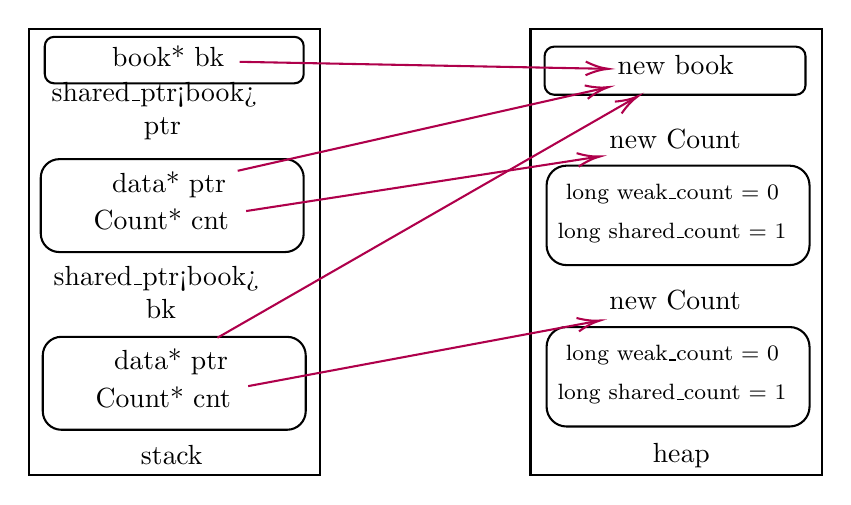
\begin{tikzpicture}[x=0.75pt,y=0.75pt,yscale=-1,xscale=1]
%uncomment if require: \path (0,300); %set diagram left start at 0, and has height of 300

%Rounded Rect [id:dp2187423114764504] 
\draw   (143.8,77.79) .. controls (143.8,72.85) and (147.81,68.84) .. (152.76,68.84) -- (261.54,68.84) .. controls (266.48,68.84) and (270.49,72.85) .. (270.49,77.79) -- (270.49,104.65) .. controls (270.49,109.6) and (266.48,113.61) .. (261.54,113.61) -- (152.76,113.61) .. controls (147.81,113.61) and (143.8,109.6) .. (143.8,104.65) -- cycle ;
%Shape: Rectangle [id:dp2941975065261839] 
\draw   (138,6) -- (278.23,6) -- (278.23,221.21) -- (138,221.21) -- cycle ;
%Shape: Rectangle [id:dp09704288189667065] 
\draw   (379.77,6) -- (520,6) -- (520,221.21) -- (379.77,221.21) -- cycle ;
%Rounded Rect [id:dp20297270277383261] 
\draw   (387.51,81.56) .. controls (387.51,76.27) and (391.8,71.98) .. (397.09,71.98) -- (504.61,71.98) .. controls (509.91,71.98) and (514.2,76.27) .. (514.2,81.56) -- (514.2,110.31) .. controls (514.2,115.6) and (509.91,119.89) .. (504.61,119.89) -- (397.09,119.89) .. controls (391.8,119.89) and (387.51,115.6) .. (387.51,110.31) -- cycle ;
%Rounded Rect [id:dp4729067946282406] 
\draw   (145.74,14.4) .. controls (145.74,11.93) and (147.74,9.93) .. (150.21,9.93) -- (266.01,9.93) .. controls (268.49,9.93) and (270.49,11.93) .. (270.49,14.4) -- (270.49,27.84) .. controls (270.49,30.31) and (268.49,32.31) .. (266.01,32.31) -- (150.21,32.31) .. controls (147.74,32.31) and (145.74,30.31) .. (145.74,27.84) -- cycle ;
%Rounded Rect [id:dp44562021942027163] 
\draw   (144.77,163.41) .. controls (144.77,158.46) and (148.78,154.45) .. (153.72,154.45) -- (262.5,154.45) .. controls (267.45,154.45) and (271.46,158.46) .. (271.46,163.41) -- (271.46,190.27) .. controls (271.46,195.21) and (267.45,199.22) .. (262.5,199.22) -- (153.72,199.22) .. controls (148.78,199.22) and (144.77,195.21) .. (144.77,190.27) -- cycle ;
%Rounded Rect [id:dp955530270440262] 
\draw   (387.51,159.32) .. controls (387.51,154.03) and (391.8,149.74) .. (397.09,149.74) -- (504.61,149.74) .. controls (509.91,149.74) and (514.2,154.03) .. (514.2,159.32) -- (514.2,188.07) .. controls (514.2,193.36) and (509.91,197.65) .. (504.61,197.65) -- (397.09,197.65) .. controls (391.8,197.65) and (387.51,193.36) .. (387.51,188.07) -- cycle ;
%Rounded Rect [id:dp3609920895859484] 
\draw   (386.54,19.27) .. controls (386.54,16.71) and (388.62,14.64) .. (391.18,14.64) -- (507.63,14.64) .. controls (510.19,14.64) and (512.26,16.71) .. (512.26,19.27) -- (512.26,33.18) .. controls (512.26,35.74) and (510.19,37.81) .. (507.63,37.81) -- (391.18,37.81) .. controls (388.62,37.81) and (386.54,35.74) .. (386.54,33.18) -- cycle ;

% Text Node
\draw (147.56,30.2) node [anchor=north west][inner sep=0.75pt]   [align=left] {shared\_ptr<book>\\ \ \ \ \ \ \ \ \ \ \ ptr};
% Text Node
\draw (176.68,73.3) node [anchor=north west][inner sep=0.75pt]   [align=left] {data* ptr};
% Text Node
\draw (167.76,91.36) node [anchor=north west][inner sep=0.75pt]   [align=left] {Count* cnt};
% Text Node
\draw (190.58,205.25) node [anchor=north west][inner sep=0.75pt]   [align=left] {stack};
% Text Node
\draw (437.22,204.47) node [anchor=north west][inner sep=0.75pt]   [align=left] {heap};
% Text Node
\draw (416.27,52.87) node [anchor=north west][inner sep=0.75pt]   [align=left] {new Count};
% Text Node
\draw (395.34,79.22) node [anchor=north west][inner sep=0.75pt]  [font=\footnotesize] [align=left] {long weak\_count = 0};
% Text Node
\draw (391.32,98.07) node [anchor=north west][inner sep=0.75pt]  [font=\footnotesize] [align=left] {long shared\_count = 1};
% Text Node
\draw (148.53,118.96) node [anchor=north west][inner sep=0.75pt]   [align=left] {shared\_ptr<book>\\ \ \ \ \ \ \ \ \ \ \ bk};
% Text Node
\draw (176.66,12.82) node [anchor=north west][inner sep=0.75pt]   [align=left] {book* bk};
% Text Node
\draw (177.65,158.91) node [anchor=north west][inner sep=0.75pt]   [align=left] {data* ptr};
% Text Node
\draw (168.73,176.98) node [anchor=north west][inner sep=0.75pt]   [align=left] {Count* cnt};
% Text Node
\draw (420.27,17.53) node [anchor=north west][inner sep=0.75pt]   [align=left] {new book};
% Text Node
\draw (416.27,130.63) node [anchor=north west][inner sep=0.75pt]   [align=left] {new Count};
% Text Node
\draw (395.34,156.98) node [anchor=north west][inner sep=0.75pt]  [font=\footnotesize] [align=left] {long weak\_count = 0};
% Text Node
\draw (391.32,175.83) node [anchor=north west][inner sep=0.75pt]  [font=\footnotesize] [align=left] {long shared\_count = 1};
% Connection
\draw [color={rgb, 255:red, 175; green, 0; blue, 75 }  ,draw opacity=1 ]   (239.66,21.95) -- (415.27,25.3) ;
\draw [shift={(417.27,25.34)}, rotate = 181.09] [color={rgb, 255:red, 175; green, 0; blue, 75 }  ,draw opacity=1 ][line width=0.75]    (10.93,-3.29) .. controls (6.95,-1.4) and (3.31,-0.3) .. (0,0) .. controls (3.31,0.3) and (6.95,1.4) .. (10.93,3.29)   ;
% Connection
\draw [color={rgb, 255:red, 175; green, 0; blue, 75 }  ,draw opacity=1 ]   (238.68,74.46) -- (415.32,34.59) ;
\draw [shift={(417.27,34.15)}, rotate = 167.28] [color={rgb, 255:red, 175; green, 0; blue, 75 }  ,draw opacity=1 ][line width=0.75]    (10.93,-3.29) .. controls (6.95,-1.4) and (3.31,-0.3) .. (0,0) .. controls (3.31,0.3) and (6.95,1.4) .. (10.93,3.29)   ;
% Connection
\draw [color={rgb, 255:red, 175; green, 0; blue, 75 }  ,draw opacity=1 ]   (228.91,154.91) -- (429.78,39.53) ;
\draw [shift={(431.51,38.53)}, rotate = 150.13] [color={rgb, 255:red, 175; green, 0; blue, 75 }  ,draw opacity=1 ][line width=0.75]    (10.93,-3.29) .. controls (6.95,-1.4) and (3.31,-0.3) .. (0,0) .. controls (3.31,0.3) and (6.95,1.4) .. (10.93,3.29)   ;
% Connection
\draw [color={rgb, 255:red, 175; green, 0; blue, 75 }  ,draw opacity=1 ]   (242.76,93.85) -- (411.29,67.85) ;
\draw [shift={(413.27,67.54)}, rotate = 171.23] [color={rgb, 255:red, 175; green, 0; blue, 75 }  ,draw opacity=1 ][line width=0.75]    (10.93,-3.29) .. controls (6.95,-1.4) and (3.31,-0.3) .. (0,0) .. controls (3.31,0.3) and (6.95,1.4) .. (10.93,3.29)   ;
% Connection
\draw [color={rgb, 255:red, 175; green, 0; blue, 75 }  ,draw opacity=1 ]   (243.73,178.2) -- (411.3,146.96) ;
\draw [shift={(413.27,146.59)}, rotate = 169.44] [color={rgb, 255:red, 175; green, 0; blue, 75 }  ,draw opacity=1 ][line width=0.75]    (10.93,-3.29) .. controls (6.95,-1.4) and (3.31,-0.3) .. (0,0) .. controls (3.31,0.3) and (6.95,1.4) .. (10.93,3.29)   ;

\end{tikzpicture}

\end{center}